\vspace{-0.2cm}
\section{Introduction}
Large language models (LLMs), including GPT Family~\citep{achiam2023gpt,dettmers2022gpt3}, LLaMA Family~\citep{touvron2023llama,touvron2023llama2,dubey2024llama3}, and Qwen Family~\citep{bai2023qwen,team2024qwen2,yang2025qwen3}, have achieved state-of-the-art performance in tasks such as commonsense reasoning, document summarization, and few-shot learning. However, these advances come at a substantial cost: LLMs with billions of parameters demand enormous computational and memory resources, rendering them impractical for deployment on edge devices.
To address this challenge, model compression has become a key research direction, with approaches such as quantization~\citep{frantar2022gptq,hu2025ostquant}, network pruning~\citep{ashkboos2024slicegpt}, knowledge distillation~\citep{hinton2015distilling}, and low-rank decomposition~\citep{yuan2023asvd,li2025adasvd}. 
Among these, low-rank compression, typically implemented through Truncated Singular Value Decomposition~\citep{Eckart1936}, directly reduces both parameter count and computational cost by factorizing weight matrices into low-rank components. This efficiency makes it particularly appealing for LLMs deployment, as the method is hardware-agnostic and can be seamlessly integrated with other compression techniques.


% \begin{figure}[htbp]
%     \vspace{-1.5cm}
%     \centering
%     % 子图 (a)
%     \begin{subfigure}[b]{0.495\textwidth}
%         \centering
%         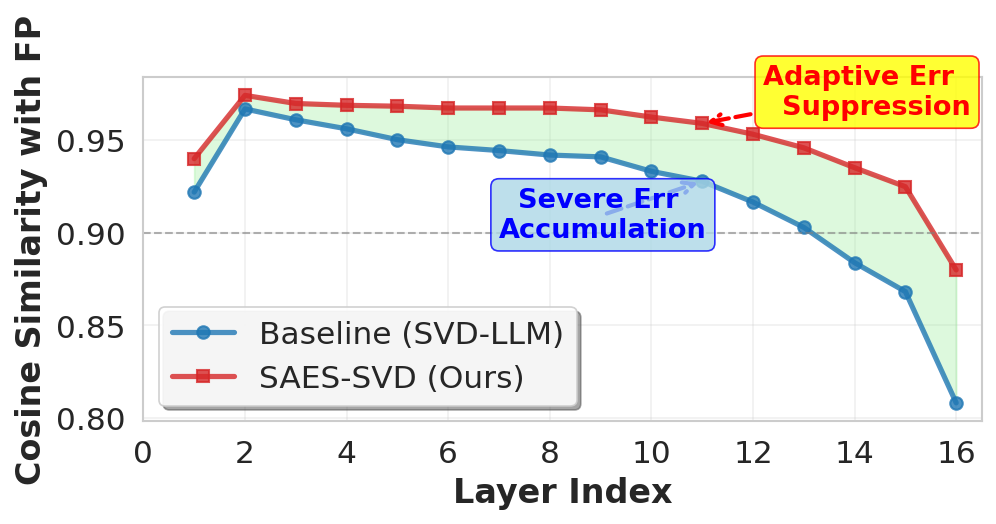
\includegraphics[width=\textwidth]{figs/error_accumulation_comparison.png}
%         \vspace{-5mm}
%         \caption{}
%         \label{fig:sub1}
%     \end{subfigure}
%     \hfill
%     % 子图 (b)
%     \begin{subfigure}[b]{0.495\textwidth}
%         \centering
%         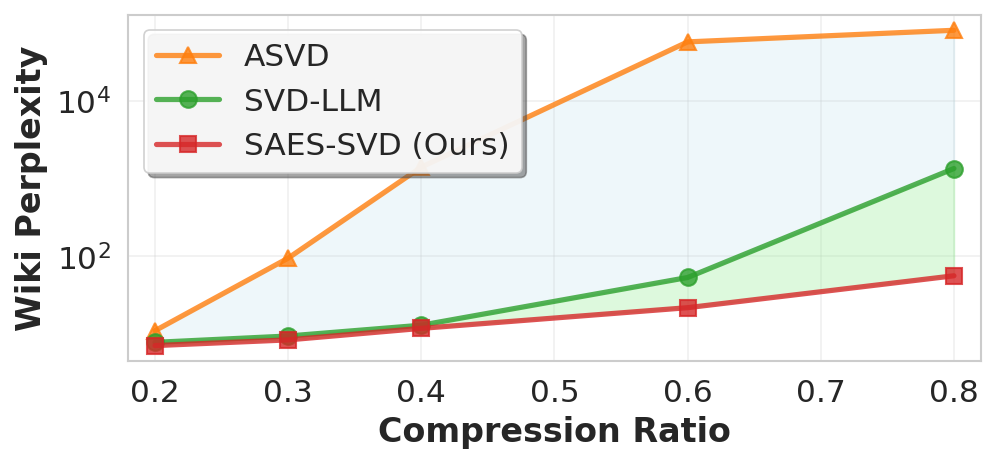
\includegraphics[width=\textwidth]{figs/perplexity_compression_comparison.png}
%         \vspace{-5mm}
%         \caption{}
%         \label{fig:sub2}
%     \end{subfigure}
%     \vspace{-0.6cm}
%     \caption{Comparison of SAES-SVD with baseline methods. 
%     \textbf{(a)} Cumulative error analysis on LLaMA-3.2-1B, showing the cosine similarity of compressed outputs with the original reference across layers. SAES-SVD effectively mitigates error accumulation by adaptively suppressing upstream deviations. 
%     \textbf{(b)} Perplexity on WikiText2 under varying compression ratios. SAES-SVD consistently achieves lower perplexity than ASVD and SVD-LLM.
%     % demonstrating robustness under high compression settings.
%     }
%     \label{fig intro}
%     \vspace{-0.2cm}
% \end{figure}


\begin{figure}[htbp]
    \vspace{-1.5cm}
    \centering

    % 子图 (a)
    \begin{subfigure}[b]{0.497\textwidth}
        \centering
        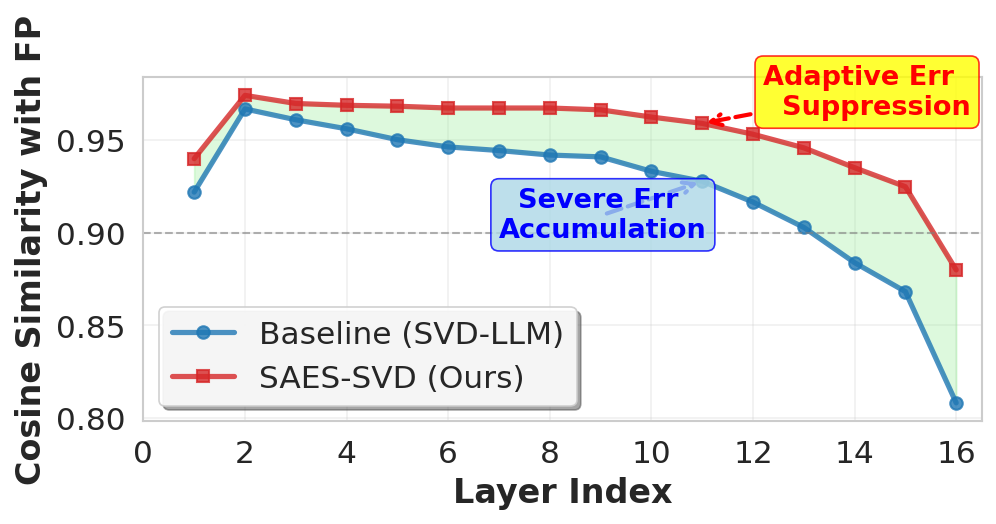
\includegraphics[width=\textwidth]{figs/error_accumulation_comparison.png}
        \vspace{-5mm}
        \caption{}
        \label{fig:sub1}
    \end{subfigure}
    \hfill
    % 子图 (b)
    \begin{subfigure}[b]{0.497\textwidth}
        \centering
        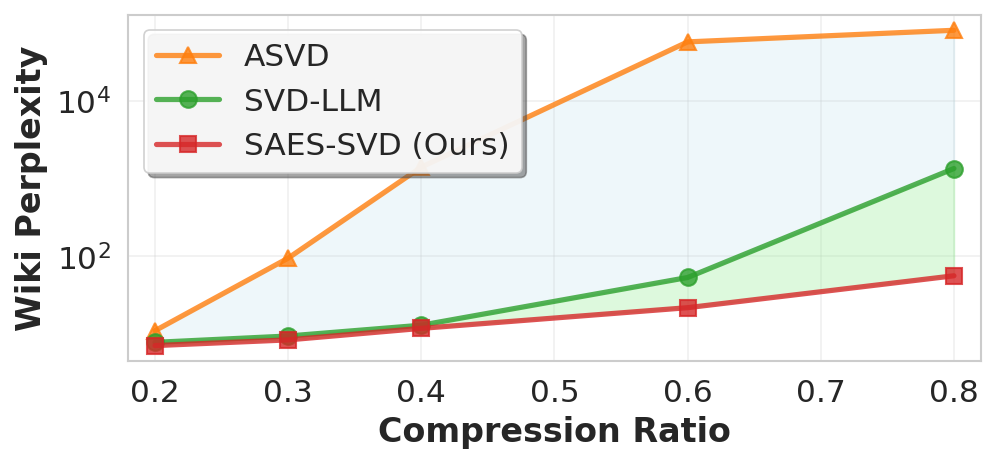
\includegraphics[width=\textwidth]{figs/perplexity_compression_comparison.png}
        \vspace{-5mm}
        \caption{}
        \label{fig:sub2}
    \end{subfigure}

    % 换行
    \vspace{-0.1cm}

    % 子图 (c)
    \begin{subfigure}[b]{0.496\textwidth}
        \centering
        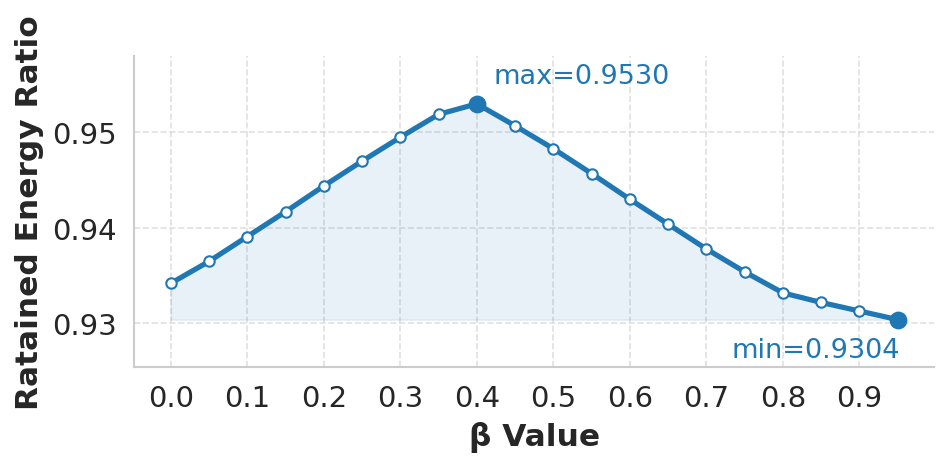
\includegraphics[width=\textwidth]{figs/ratio_of_differnet_beta.png}
        \vspace{-5mm}
        \caption{}
        \label{fig:sub3}
    \end{subfigure}
    \hfill
    % 子图 (d)
    \begin{subfigure}[b]{0.496\textwidth}
        \centering
        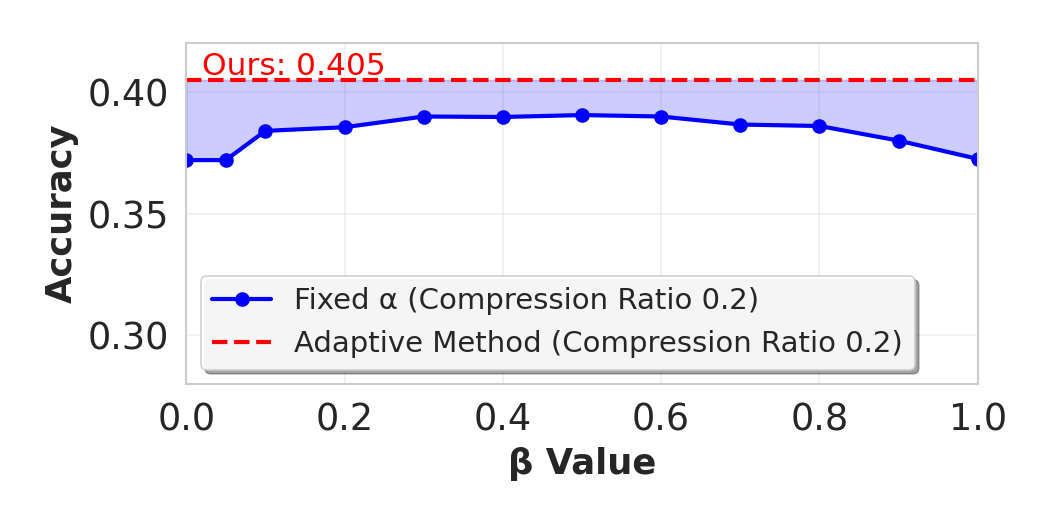
\includegraphics[width=\textwidth]{figs/3_plot_different_alpha.png}
        \vspace{-5mm}
        \caption{}
        \label{fig:sub4}
        \label{fig different alpha}
    \end{subfigure}
    \vspace{-0.6cm}
    \caption{
    \textbf{(a)} Cumulative error analysis on LLaMA-3-8B, showing the cosine similarity of compressed outputs with the original reference across layers. SAES-SVD effectively mitigates error accumulation by adaptively suppressing upstream deviations. 
    \textbf{(b)} Perplexity on WikiText2 under varying compression ratios. SAES-SVD consistently achieves lower perplexity than ASVD and SVD-LLM.
    \textbf{(c)} Retained Energy Ratio achieved by using different weighting coefficients for the cumulative error compensation term in with rank=128 compression for k-proj in the 14th Layer of LLaMA-3-8B. Here, for the sake of convenience, we use $\beta=\alpha/(1+\alpha)$ as the horizontal axis.
    \textbf{(d)} Effect of fixed versus adaptive weighting coefficients for the cumulative error compensation on average accuracy across 7 zero-shot benchmarks.
    }
    \label{fig:intro}
    \label{fig intro}
    \vspace{-0.2cm}
\end{figure}


Existing low-rank compression methods typically focus on layer-wise optimization. For example, methods such as ASVD~\citep{yuan2023asvd}, SVD-LLM~\citep{Wang2024SVD-LLM}, and AdaSVD~\citep{li2025adasvd} aim to reduce local reconstruction error within individual layers by introducing activation-aware scaling, applying whitening transformations, and performing adaptive iterative refinement, respectively.
However, these approaches share a fundamental \textbf{limitation: they tend to minimize the reconstruction error for each layer independently, without considering how errors propagate and accumulate through the network.} In practice, reconstruction errors from early layers alter the input distribution of subsequent layers, causing these errors to compound and leading to an increasingly larger gap from the full-precision baseline.
Applying SVD-LLM~\citep{Wang2024SVD-LLM} to LLaMA2-7B further supports this observation. Although SVD-LLM achieves the theoretical minimum truncation error at each layer, the similarity to full-precision outputs, as shown in Figure~\ref{fig:sub1}, decreases steadily from 0.97 to 0.79 across layers. This result indicates that minimizing per-layer reconstruction error alone does not guarantee end-to-end fidelity.

Building on these observations, we propose Self-Adaptive Error Suppression SVD (SAES-SVD), a low-rank compression framework that incorporates cumulative error compensation into the optimization objective. The core idea of SAES-SVD is to let each layer perceive accumulated compression errors from previous layers and adapt its compression strategy based on its sensitivity to those errors. In this way, conventional independent layer-wise optimization is transformed into a globally coordinated error-suppression mechanism. Specifically, SAES-SVD consists of two main components:
\ding{182} \textbf{Cumulative Error-Aware Layer Compression (CEALC):} For each layer, we minimize not only the local reconstruction error but also enforce alignment with the corresponding full-precision reference. This alignment helps compensate for errors propagated from upstream compressed layers. The dual objective is formulated as a weighted Frobenius norm of reconstruction and alignment errors. From this objective, we derive a closed-form solution that effectively suppresses reconstruction error and compensates for cumulative error. Moreover, it achieves this with only minimal additional cost, as the method relies solely on second-order statistics of activation deviations and a few extra matrix operations compared with vanilla SVD compression.
\ding{183} \textbf{Adaptive Collaborative Error Suppression (ACES):} Since each layer has different sensitivity to compression ratio and cumulative error, using a fixed weighting coefficient (i.e., $\alpha_\ell$ in Equation~\ref{eq:initial}) for cumulative error compensation often results in suboptimal solutions. As shown in Figure~\ref{fig:sub3}, varying the coefficient across layers leads to different values of the Retained Energy Ratio (RER), defined as the proportion of the squared sum of the top-$k$ singular values to the total squared sum after SVD. RER serves as a measure of the low-rank structure of the compression objective, where a higher RER indicates stronger energy concentration in the leading singular values and thus greater compression efficiency. To address this issue, we introduce an adaptive weighting coefficient for each layer (i.e., $\beta_\ell^*$ in Equation~\ref{eq:beta obj}). The coefficient is automatically tuned to maximize RER. By concentrating energy on the dominant singular values, this optimization yields compact and informative low-rank representations and enables energy-aware error compensation that improves compression efficiency under fixed rank budgets.

We conducted a comprehensive evaluation of SAES-SVD across diverse datasets, model architectures, and representative SVD-based baselines. The evaluation included language modeling, classification, and generation tasks. Results from multiple benchmarks, such as Figure~\ref{fig intro}, show that SAES-SVD effectively suppresses cumulative errors introduced during compression. Figure~\ref{fig:sub1} indicates that cosine similarity with full-precision outputs remains consistently higher across layers. Figure~\ref{fig:sub2} and Figure~\ref{fig:sub4} further shows that SAES-SVD achieves much lower perplexity and higher accuracy under diverse compression ratios. 
The main contributions of this work are threefold:
\setlength{\leftmargini}{10pt}
\vspace{-3mm}
\begin{itemize}
    \item
    We identify that independent layer-wise compression leads to the amplification of cumulative errors. To address this, we propose CEALC, which moves beyond independent optimization and explicitly incorporates cross-layer error accumulation into the low-rank objective. Building on this formulation, we derive an efficient closed-form low-rank solution that depends only on second-order activation statistics. 
\vspace{-1mm}
    \item 
    We introduce ACES, which use an adaptive coefficient $\alpha$ to control the weighting of cumulative error compensation. The value of $\alpha$ is adjusted to maximize the proportion of retained energy. This optimization enhances the low-rank structure of the compression objective and ensures that, under a fixed rank budget, the retained components preserve as much information as possible.
\vspace{-1mm}
    \item 
    CEALC and ACES together form the framework SAES-SVD. Experiments demonstrate that SAES-SVD is both effective and broadly applicable. At the 20\% compression ratio, without requiring complex rank allocation or additional fine-tuning, it reduces the drop in zero-shot accuracy by 58\% and lowers the perplexity gap by 52\% compared with Dip-SVD. These improvements substantially narrow the gap between the compressed model and the full-precision baseline.
\end{itemize}

